%
% File acl2014.tex
%
% Contact: giovanni.colavizza@epfl.ch
%%
%% Based on the style files for ACL-2013, which were, in turn,
%% Based on the style files for ACL-2012, which were, in turn,
%% based on the style files for ACL-2011, which were, in turn, 
%% based on the style files for ACL-2010, which were, in turn, 
%% based on the style files for ACL-IJCNLP-2009, which were, in turn,
%% based on the style files for EACL-2009 and IJCNLP-2008...

%% Based on the style files for EACL 2006 by 
%%e.agirre@ehu.es or Sergi.Balari@uab.es
%% and that of ACL 08 by Joakim Nivre and Noah Smith

\documentclass[11pt]{article}
\usepackage{acl2014}
\usepackage{times}
\usepackage{url}
\usepackage{latexsym}
\usepackage{graphicx}
\usepackage[font=small,skip=2pt]{caption}
\usepackage{float}

%\setlength\titlebox{5cm}

% You can expand the titlebox if you need extra space
% to show all the authors. Please do not make the titlebox
% smaller than 5cm (the original size); we will check this
% in the camera-ready version and ask you to change it back.


\title{A study on Amazon's distinctive features}

\author{Raphael Barman \\
  {\small \tt raphael.barman@epfl.ch} \\\And
  Hakim Invernizzi \\
  {\small \tt hakim.invernizzi@epfl.ch} \\\And
Albane Descombes \\
{\small \tt albane.descombes@epfl.ch} \\}

\date{}

\begin{document}
\maketitle
\begin{abstract}
 Can we really trust the Amazon's underlying system? This document describes and discusses the results obtained in the context of the authors' project in ADA2017. The project aims at deepening the understanding 
  of Amazon's whole system. Particular attention is put into detecting if the system seems to be used correctly or if there's a general bias.\par
  Three major results were produced.
  First, we found out that users tend to rate very high with low variation. Secondly, it was noted that Amazon's 'also bought' and 'bought together' features played a big role in the ranking of the products. Finally, we also found that the more a category has reviews, the less helpful they tend to be.
\end{abstract}


\section{Introduction}
  The analysis is centered around three different aspects.\\ First, the review feature, with the goal to describe its usage from the userbase and answer the question of whether reviews are generally biased or not. \par 
 Second, the adverting feature which is composed of the "also bought", "also viewed" and "bought together" features. The intra-correlation among the sub-features as well as their impact on the whole system are the subject of study. \\
Lastly, the categorization feature and its impact on the user perception of a product. \\ 
The three features represent three different starting points for the analysis which should ideally converge in a single conclusion about bias.
  
\section{Related work}
Past researches focused on the relationship between product quality and the reviews and tried to find if there were some metrics that would help predicting the product quality from the reviews \cite{hu2006can}. Other researchers tried to find the link between helpfulness and other metrics and found results that were strongly tied with the categories of the products \cite{mudambi2010makes}. Finally some studies found out that user reviews were strongly biased and that they could be easily manipulated through some herding effect \cite{muchnik2013social}.

\section{Data collection}
All the data comes from the Amazon product dataset created by James McAuley \cite{mcauley2015image}.\\
 The goal was to use a quite large sample having a significant number of reviews per user and per product, thus the 5-core dataset was chosen. This dataset guarantees reviews with a minimum of 5 reviews per reviewer and 5 reviews products. The size is in the magnitude of the 18 millions.
\section{General data description}
The features of the data relevant for the analysis are the following: the ID of the reviewer that is a unique ID, the ID of the product that is found in both the review and in the metadata, the text of the review that allows to make a word count, the helpfulness of the review that is given in the form of [number of people that found the review useful, number of people that vote] and finally the actual rating given in the review.\par
 Concerning the metadata, its usage is to help understand more about the Amazon's system. The most relevant features are the "related" features that comprises "also viewed" and "bought together" that gives some insight about how Amazon recommends particular products. Another interesting feature is the sales rank feature that gives some insight of the popularity of a product and comports both the rank of the product and the category of the ranking.

The dataset we used is composed of 18186733 reviews from 1116318 unique reviewers that reviewed 731283 unique products. The histogram of the rating (see figure \ref{rating_hist}) shows that most of the reviews have a very high rating.
\begin{figure}[H]
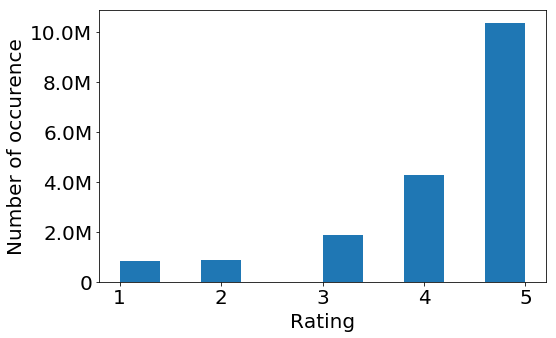
\includegraphics[width=0.5\textwidth]{rating_hist.png}
\caption{Histogram of the ratings}
\label{rating_hist}
\end{figure}

There is no missing data for the review concerning the features mentioned above.
Concerning the metadata, the category and the rank is missing in 35\% of the products and the "related" features are missing in between 65 to 75 \% of the products. This has to be kept in mind when those features are used.
\section{Analysis}
\subsection{Review feature}
    The first step in trying to describe Amazon's reviews was trying to detect potential correlation between its features. This was done by defining two metrics: the "wordcount", which is 
  the length of a review in number of words, and the "helpfulness", which is a user-defined measure of the usefulness of a review in the range [0, 1]. By observing the distribution of these two metrics it was possible to remark that the majority of reviews are less than 1000-words long and that their average helpfulness is high.\\ The correlation between these two metrics and  other descriptive features of the review was then studied. The only relevant result was noticing the presence of a weak Spearman correlation (0.29) between helpfulness and the review's rating of the product. This hint at the presence of a monotonic component in the relationship, meaning that if a review gives a high rating to the review product then the review is slightly more likely to be judged as helpful. This is not the expected behaviour of the relationship, as the product rating of a review and its helpfulness should be independent variables.
\begin{figure}[h]
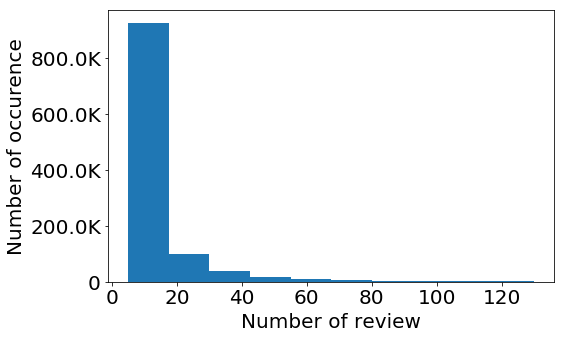
\includegraphics[width=0.5\textwidth]{review_user.png}
\caption{Histogram of number of review per user}
\label{reviews_per_user}
\end{figure}

The second step was trying to quantify the bias from the reviewers. A first analysis showed that the average number of reviews written per user is low (see figure \ref{reviews_per_user}). The average rating for each reviewer was computed, then further averaged to obtain the mean average rating. This value is of 4.24 out of 5, with a mean standard deviation of 0.86. It can be argued that the mean average rating is high while the mean standard deviation is low. Furthermore by varying the sample based on the standard deviation, it was noted that the weaker the standard deviation, the higher the average for the reviewer (see figure \ref{rating_users_std_025}).
\begin{figure}[h]
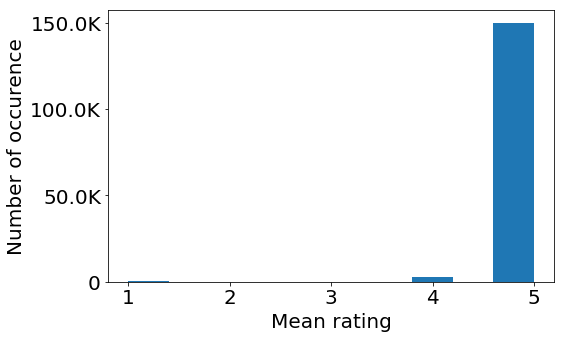
\includegraphics[width=0.5\textwidth]{rating_std025.png}
\caption{Histogram of the user average rating with an average std $<$ 0.25}
\label{rating_users_std_025}
\end{figure}

This is a peculiar result that could be argued as pointing towards a general bias in the review system, since the only situation that justify these results is that all products are excellent, an hypothesis which doesn't hold. A possible explanation to this behaviour could be that Amazon users  tend to rate the product they're satisfied with and not those they're unsatisfied with.\\\\
The third step was studying the users behaviour with regard to the brand. The approach was to select reviewers with at least 5 reviews concerning the same brand and analyze the mean average rating and mean standard deviation. These values are 4.29 and 0.74 respectively. The small decrease in the mean standard deviation is not enough to draw any conclusion, therefore it will be assumed that the user aren't biased towards brands.\\\\
Furthermore, the correlation between the ranking of a product and its reviews' quantity, average helpfulness and average rating were studied without meaningful results.

\subsection{Advertising features}
  The three advertising features subject of the study are the "also bought", "bought together" and "also viewed" features. As a first approach, correlation between these three features and the product ranking have been computed. While there were no relevant results concerning "also viewed", Spearman correlations of 0.56 and 0.45 have been detected in the relationships between the ranking of two product that were part of the "bought together" and "also bought" feature respectively. These results imply the presence of a monotonic component in the ranking of 'bought together' and 'also bought' items, which means the ranking of one product influences the ranking of the other. \\\\
Another goal of the research was to examine the intra-correlation between the three features, however due to the array-like nature of these attributes and the consequent exponential growth in the size of the Dataframe, this was not feasible.

\subsection{Categorization feature}
The third part of this analysis aims at assessing the impact of the product categorisation on the whole Amazon's system. To do this, products are divided by category. Then, the number of reviews per category as well as the average helpfulness and average product rating per categories are computed.\\
Please note that Amazon has two parallel product categorisation systems: one that is used for the product ranking, and a second one which is descriptive in nature.\\\\
For both categorisation systems, it was found that categories which are conceptually broader ("Automotive") have many more reviews compared to niche category ("Pizza Kits"). The mean average helpfulness is 0.89, highlighting the fact that the usefulness of the reviews is judged in a positive way. Concerning the mean average rating, it is close to 3.98, a result which is lined with the result obtained in the analysis of reviews.\\\\
Furthermore, there are interesting results from the point of view of Spearman correlations.\\
Concerning the ranking categorization system, a correlation of 0.41 was found in the association of the average helpfulness and average product ranking. This means that there's a weak monotonic component in this relationship, similarly to what was observed in the first part of this analysis. Furthermore, the correlation between average helpfulness and number of reviews per category is -0.35. The interpretation of this result is that if a category has many reviews, then it is slightly less likely that the reviews are considered helpful in average. \\
Concerning the general categorization system, there's a common moderate correlation between average helpfulness and number of reviews per category (-0.45), which can be interpreted as described above.

\section{Conclusion}
In the first step of the analysis, a weak correlation among the helpfulness and product rating of a review was detected, when theoretically they should be independent variables. Mean helpfulness is high (0.9). It was also noted that the mean average product rating was high (4.24 out of 5) and the mean standard deviation was low (0.86), facts that lead to think that users tend to favour giving high ratings. This was enforced when noticing that the smaller the standard deviation, the higher the mean average rating in the study sample. \\
This result is peculiar because it is hard to believe that this data really reflects the quality of the observed Amazons's products. The mean average product rating is too high: supposing that low quality products also exist, it should be more towards 3.0. 
\\A possible explanation is that users tend to review the product they're satisfied with, and are less diligent in rating the product they're not satisfied with. This behaviour would bias the data and produce data similar to the ones we observed.\\\\
In the second part of the analysis, two relevant results were produced: two moderate correlations (0.56, 0.41) between the ranks of products that were bought together. This speaks of a "boost" factor in the ranking of certain products, which gained positions by benefiting from the influence of a higher ranked product. This is not a form of user bias per se, but it's most likely  a bias voluntarily introduced with the "bought together" and "also bought" features, which suggests users to buy products that other users bought together with the observed one. Unfortunately, it was beyond our capabilities to examine the correlation between the "bought together" and  "also bought"  features, which would have allowed to add informations to the picture.\\\\
In the third part of the analysis, the correlation between average helpfulness and average rating was confirmed to hold even if these values are computed per ranking category. The interesting result produced is the correlation between the number of reviews and the average helpfulness of reviews in a category (-0.35 for ranking categories, -0.45 for general categories). The interpretation of this result is that if a category has many reviews, then it is less likely that the reviews are considered helpful in average. This might makes sense, because if many reviews are available, then the user can use a comparative approach in choosing which review is most helpful; however when there's few review, the lack of information brings the user to lower its standards in appreciation. \\\\

In light of these observations, it can be affirmed that bias plays a role in the Amazon's system: may it be user introduced bias as seen in the first part, or "design bias" as seen in the second part, or even bias due to a lack of information as seen in the third part.
\newpage
\bibliographystyle{acl}
\bibliography{bibliography}

\end{document}
